\chapter{Overall Description}
\section{Product Perspective}
\subsection{Scenarios}

\subsubsection{Creating a tournament}
Chip, a professor of Algorithm and Data Structures at Mouseton Institute of Technology prepared to teach the chapter on strings, launching the "Strings Operations" coding tournament on CKB.
To expand participation, he allowed his colleague Dale to create challenges for his software engineering class.
Students across classes would compete in string manipulation tasks, ranging from basic concatenation to advanced text analysis, fostering collaboration and learning.
To make the tournament more interesting, Chip decided to award badges to the best-performing students, so he added badges for the students who participate in most tournaments, one for the students who win most battles, and one for the students who write most lines of code.
All students already subscribed to CKB were notified of the new tournament, and they could join it from the tournament page till a defined deadline.

\subsubsection{Creating a battle}
In order to familiarize students with the CKB platform and its features, Chip created an easy battle for his students to practice, called 'Wordcheck.' 
The task essentially required students to implement the game Wordle in the C language. 
He decided that the battle would last for two weeks, allowing students to work in teams of 2 or 3 people. Students would be able to join the battle until its last day.
\\ {\color{red} La finestra di registrazione può overlappare con il tempo della battaglia / Una conseguente all'altra} \\
In addiction, he wanted to give extra points for code cleanup. 
Therefore, he had to review the code of each team at the end of the battle and assign extra points to the teams that wrote clean code. 
Chip set all this information in the battle creation form and then created the battle.

\subsubsection{Joining a battle}
Huey and Dewey, two students of Chip's class, are notified of an incoming battle and decide to join it.
Since the more the merrier, they decide to invite their friend Louie to join them in the battle.
Louie receives the invitation mail and decides to join the battle in their team.
After the registration deadline, they are notified that the battle is about to start.
They get the link to the GitHub repository of the battle to fork it and then set up an automated workflow to link their GitHub account to the CKB platform.
\\ {\color{red} In contrasto con la cosa scritta sopra per la finestra e l'inizio battaglia} \\
After the automated workflow is set up, they are ready to start working on the battle.

\subsubsection{Improving the score and obtaining a badge}
Donald is another warrior of the "Wordcheck" battle and he is working on the battle alone.
\\ {\color{red} Non può partecipar da solo per i vincoli definiti dal prof sopra} \\ 
After the first commit, he logs in to the CKB to check his score.
He sees that he is in the 3rd position and that he is 10 points behind the leading team, composed by Huey, Dewey and Louie.
Fortunately, the battle is still in progress and the CKB platform allows him to improve his score by pushing new commits to the GitHub repository, so he decides to work on the battle for a couple of days and then push his updated work to the GitHub repository.
After checking his score again, he is now in the 1st position and moreover he obtained a badge for being the first to reach 100 points in the battle.
From now, both students and professors can see this badge when they visit Donald's profile.

\subsubsection{Closing a battle}
{\color{red} Scrooge non ha avuto permessi per creare la battaglia, la battaglia Wordcheck l'ha creata Chip} \\
When the deadline for the battle created by Scrooge is reached, all participants are notified that the battle is closed and that they can not push new commits to their GitHub repository.
Scrooge is notified that the battle is closed and he can now evaluate the code of each team and assign extra points for the clarity of the comments and the code, as he decided when he created the battle.
\\ {\color{red} Non abbiamo parlato negli use cases della notifica per il prof per dirgli che la battaglia è finita e deve valuatre il codice} \\
After the evaluation, the final rank of the battle is available to all participants and the students are notified that they can now see the final rank of the battle.

\subsubsection{Closing a tournament}
Chip decides to close the "Strings Operations" tournament, when all the battles end.
In order to do so, he logs into the CKB platform and he closes the tournament.
All participants are notified that the tournament is closed, in the end, the CKB platform makes the final rank of the tournament available to all participants.

\subsubsection{Accessing the scores of the players}
Huey wishes to enroll to the class of Advanced Algorithms and Data Structures held by professor Pippo, so he applies for the class.
Pippo, who wants to make sure that Huey is a good student, comes to know that Huey is a very active user of the CKB platform and he decides to check his profile.
He sees that Huey has a very high score in the "Strings Operations" tournament and that he has a badge for being the most active user of the platform and he also notes that Huey is involved in more than one tournament simultaneously.
Thanks to the CKB platform, Pippo has now a complete overview of Huey's skills and he can decide whether to accept his application or not.

\subsubsection{Creating Game badges}
Scrooge, a Software Engineering professor at Duckburg University, believes that, in addition to the existing badges in CKB platform, it would be nice to introduce badges for students who achieves a perfect score in a battle and in a tournament.
Since the CKB platform allows educators to create new badges, he creates the two badges and from now on, all educators will have the option to include these badges in their tournaments and battles.

\subsection{Class Diagram}
{\color{red}{AGGIUNGERE classe testcase. TOGLIERE TeamScore, è uguale a ranking in battle. Togliere creates battle da educator, ridondante}} \\
In figure \ref{fig:class-diagram} is represented the class diagram of the software. 
In particular, the most important details are:
\begin{itemize}
    \item There are only two possible types of users: Student and Educator type.
    \item Educators can create tournaments and battles, moreover they can grants permission to create battles to other colleagues inside their own tournament.
    \item Students can subscribe to tournament and battles, invite other students to form teams, achieves badges, using both CKB platform and GitHub. 
          The most important detail is subscribing to a battle: a student can join a battle by creating its own team (a team is composed by at least one person, respecting imposed boundaries) or by joining an existing team. 
          In particular, the team class exist iff a battle exist, i.e. a team exists only in the battle scope.
    \item Tournament and Battle classes use the MailAPI to notify students about events.
\end{itemize}

\begin{figure}[H]
    \centering
    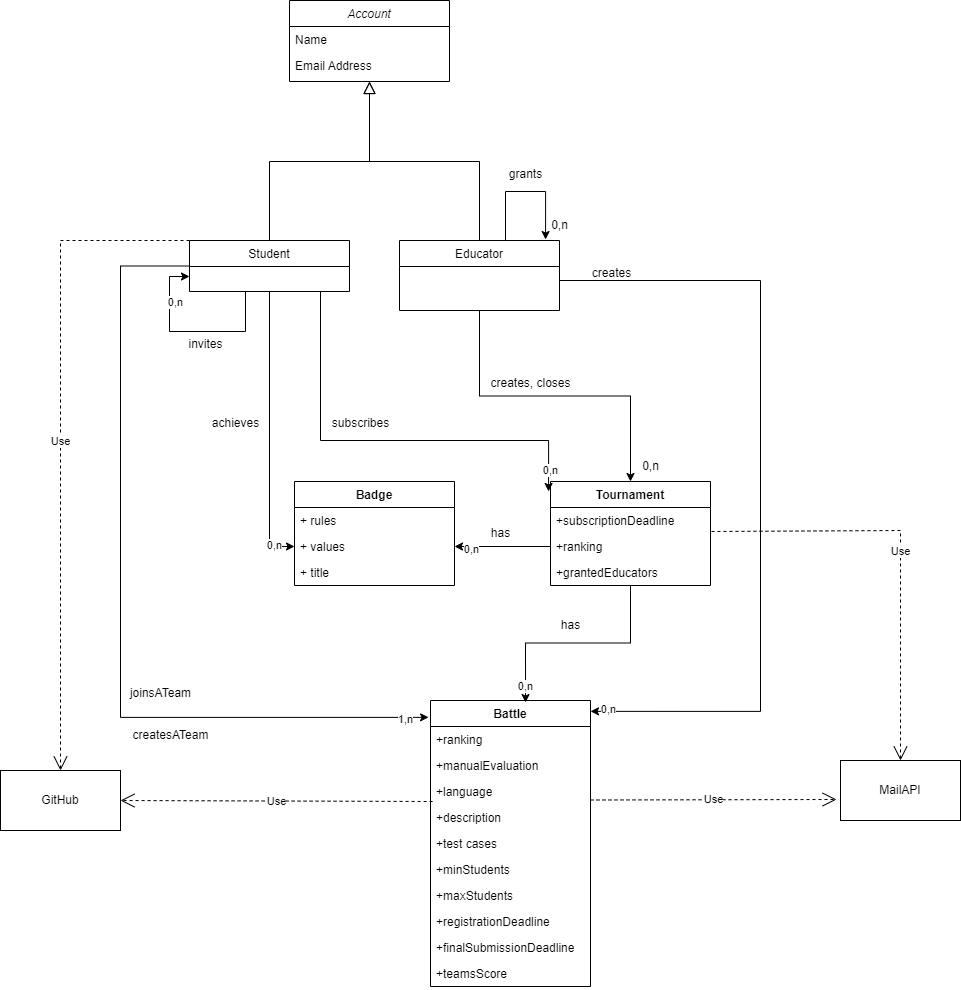
\includegraphics[width=0.8\textwidth]{images/state_diagrams/ClassDiagram.png}
    \\ {\color{red} Non direi software class diagram perchè siamo ancora nei requisiti} \\
    \caption{Class Diagram}
    \label{fig:class-diagram}
\end{figure}

\subsection{State Diagrams}
The following state diagrams describe the life cycle of the main entities of the system.
Moreover, they also specify the sequence of states that an object goes through during its lifetime in response to stimuli from the environment.
We want to focus on the events that cause a transition from one state to another and the actions that result from a state change.

\subsubsection*{Tournament}
After an educator creates a tournament, it is both in the \textit{registration open} and \textit{tournament open} states.\\
In the \textit{registration open} state, students can join the tournament, while in the \textit{tournament open} state, educators with the right permissions can create battles within the tournament, and that leads the tournament to the \textit{battling} state.\\
When the deadline for the registration is reached, the tournament moves to the \textit{registration closed} state and no more students can join it.\\
When the deadline for the registrations is reached, no more students can join the tournament and it moves permanently to the \textit{registration clcsed} state.\\
During the \textit{battling} state educatos can start multiple parallel battles and, if and only if all battles are ended, the educator can finally close the tournament.\\
The diagram is shown in figure \ref{fig:tournament-state-diagram}.

\subsubsection*{Battle}
The battle evolves in a linear way, starting from the \textit{registration opem} immediately followed by the \textit{registration closed} state.\\
After the registration deadline is reached, the github repository of the battle is created and thus the battle moves to the \textit{coding} state, allowing the students to fork the repository and start working on the battle.\\
When the deadline for the battle is reached, the educators can start evaluating the code of the students, if previously enabled (\textit{consolidation} state). \\
After the evaluation is completed, the battle can be closed and the final rank is available to all participants.\\
The diagram is shown in figure \ref{fig:battle-state-diagram}.

\subsubsection*{Score evaluation}
The score evaluation of a battle is a process that is triggered by the end of a battle and it is composed by multiple steps.\\
First, three aspects can be automatically evaluated: functional aspects (the higher the better, +), timeliness (the lower the better, -) and quality level of the sources, extracted through static analysis tools (+). \\
Finally, if the educator enabled the manual evaluation, he can assign extra points. \\
The diagram is shown in figure \ref{fig:score-evaluation-state-diagram}.

\begin{figure}[H]
    \centering
    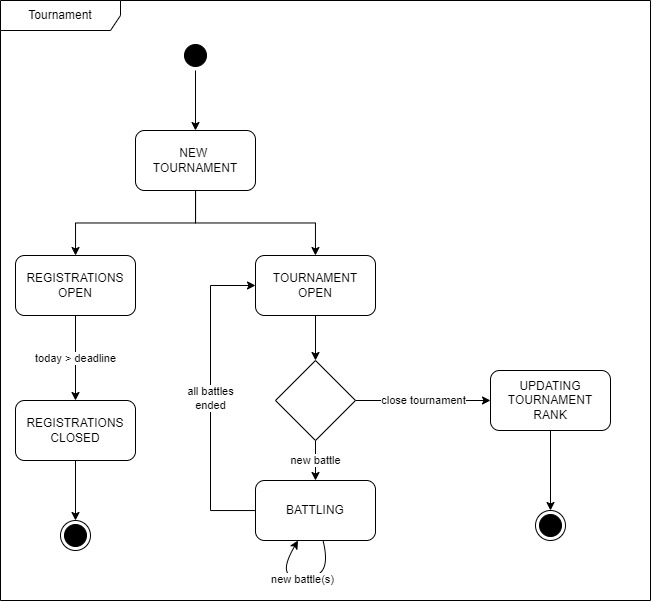
\includegraphics[width=.8\textwidth]{images/state_diagrams/tournament.jpg}
    \caption{Tournament state diagram}
    \label{fig:tournament-state-diagram}
\end{figure}
\begin{figure}[H]
    \centering
    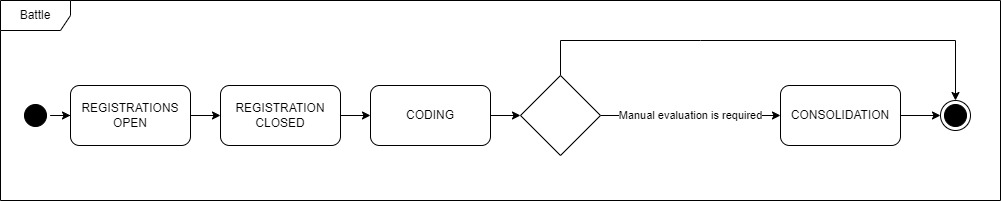
\includegraphics[width=1\textwidth]{images/state_diagrams/battle.jpg}
    \caption{Battle state diagram}
    \label{fig:battle-state-diagram}
\end{figure}
\begin{figure}[H]
    \centering
    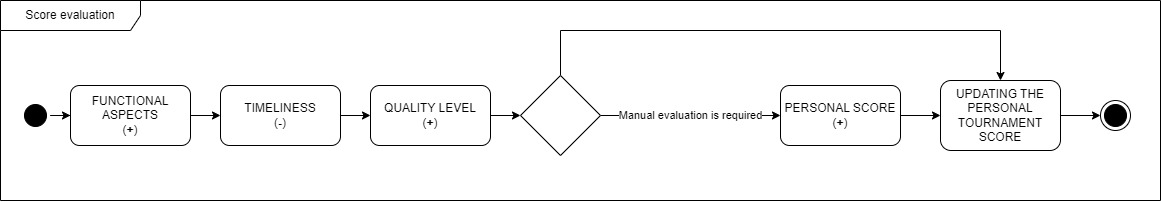
\includegraphics[width=1\textwidth]{images/state_diagrams/score_evaluation.jpg}
    \caption{Score evaluation state diagram}
    \label{fig:score-evaluation-state-diagram}
\end{figure}

\section{Product Functions}
\subsection{Register function}
A user approaching CKB for the first time can register on the platform.
The information necessary for the system to keep track of users are personal data such as Name, Surname, Email, School they belong to, and what role they hold in the school environment.
This last information is very important as it guarantees two types of accounts with different rights and duties.

By expressing that it is an EDU, all rights related to the creation of tournaments, battles, and badges will be guaranteed.
By choosing a STU account, you will be able to actively participate in tournaments and battles by earning badges.

\subsection{Create tournament function}
To create a tournament, an educator registered in CKB platform must define all the information necessary for its generation.
The tournament requires:
\begin{itemize}
    \item a name
    \item a time window aimed at welcoming student registrations
    \item a list of badges that students can obtain during the whole tournament duration
\end{itemize}

\subsection{Creating battles function}
In the context of an active tournament, any authorized EDU can decide to create a battle.
New battles require:
\begin{itemize}
    \item The programming language required to solve the problem
    \item The test cases that must be passed at the end of the battle by each team's code
    \item The build automation scripts correctly set
    \item The specification of the problem to be solved including at least one example in order to achieve test-first approach
    \item The deadline for the battle registration period
    \item The deadline for the conclusion of the battle
    \item The choice of the evaluation method, in particular, if it can choose manual evaluation in addition to the automatic one performed by the platform
    \item Constraints for the maximum and minimum number of players required for each team
\end{itemize}

\subsection{Join tournament and battles function}
Students registered on the platform receive notification every time a new tournament is created and can decide whether to participate.
Likewise, in the context of a tournament in which they applied, they are informed of new battles.
Registration for a battle can be done in various ways as long as it is before the end of the registration window.

\subsection{Gamification function}
Educators, at any time, can create a new badge by defining a title and a rule. 
Once a badge is created, it will be available on the CKB platform for every educator who wishes to use it in a new tournament. 
When creating a tournament, the educator specifies the list of included badges from those available. 
At the end of the tournament in which they are enrolled, students receive all the badges for which the specified rule has been satisfied.

\section{User characteristics}
Users of the system fall into one of the following categories: student or educator.

\subsection*{Student}
Student participates actively in code kata tournaments and battles to enhance their software development skills. 
During a battle, students develop solutions following the "test-first" approach and use GitHub to manage the code. 
The CKB platform automatically evaluates student progress based on the number of tests passed, timeliness, quality of code, providing scores updated in real-time. 
Students aim to achieve high scores and accumulate gamification badges defined by educators. 
In addition to participating in battles, students can view their tournaments' rank and receive notifications on final results. 
The student's primary goal is to improve programming skills, obtain competitive scores, and earn badges through active participation in the collaborative context of the CKB platform.

\subsection*{Educator}
The educator takes a central role in directing students toward improving software development skills through programming battle competitions. 
Its duties include creating tournaments and competitions, finalizing challenge details, and managing student registrations. 
The educator assigns specific tasks, manually evaluates students' solutions, and contributes to the automatic evaluation of projects, considering functional, temporal, and code quality aspects. 
Furthermore, it can create gamification badges, motivating students with personalized rewards based on rules it establishes. 
The main objective is to improve students' skills, ensuring fair and efficient assessment and encouraging active involvement. 
The educator plays a key role in educational innovation, exploring new possibilities through the definition of personalized rules and badges that stimulate growth and collaboration. 
In summary, the educator acts as a promoter of an engaging and competitive training challenge on CKB.

\section{Assumptions, Dependencies and Constraints}

\subsection{Domain Assumptions}
\newlist{assumptionsenumerate}{enumerate}{1}
\setlist[assumptionsenumerate,1]{label=\textbf{D}\arabic*., ref=D\arabic*}
\begin{assumptionsenumerate}
    \item STUs code with the programming language set for the battle to which they are partecipating
    \item EDUs upload the code kata with the description and the correct software project, including test cases and build automation scripts relate to it
    \item STUs fork the GitHub repository of the code kata and set up an automated workflow through GitHub Actions that informs the CKB platform (through proper API calls) as soon as STUs push a new commit into the main branch of their repository
    \item EDUs manual evaluation range from 0 to 100\footnote{The full evaluation will be given by the average of all the four aspects evaluated by the CKB platform, the three automatic ones and the manual one}
    \item The information inserted at registration moment of all users are truthful
    \item GitHub and the tool for static analysis work properly
    \item A team is formed by at least one person up to the maximum number defined by EDUs.
    \item All users subscribed to the CKB platform have a GitHub account
\end{assumptionsenumerate}

\subsection{Dependencies}
\begin{table}[H]
    \centering
    \renewcommand{\arraystretch}{1.5}
    \begin{tabular}{l l p{11.5cm}}
        \hline
        \textbf{Dep1} &  & The system will require internet connection to interact with CKB and other users           \\
        \textbf{Dep2} &  & The system will integrate an external API in order to compile the code written by students \\
        \textbf{Dep3} &  & The system will integrate a GitHub API in order create repository for each battle          \\
        \hline
    \end{tabular}
    \caption{Dependencies}
\end{table}

\subsection{Constraints}
\begin{itemize}
    \item The software must follow local laws and rules, especially when it comes to handling user data, like letting users access their data when they want.
    \item The software should only collect the data it really needs, like just the user's email address.
    \item To keep users' important info safe, like passwords and personal data, it must be stored in SHA256 encoding in the database.
    \item When choosing external APIs, especially those that are crucial for it to work properly, we should pick the ones that are the most dependable and always available.
\end{itemize}